\section{Inštalácia operačného systému}
\paragraph{}
Ako operačný systém pre servery sme nainštalovali Windows Server 2016 x64. Pre desktopy sme použili už predinštalovaný virtuálny stroj s Windows 7 x64.

\paragraph{}
Windows Server sme v rámci VirtualBox-u nastavili rovnako ako pri Debian-e s tým rozdielom, že sme namiesto "Debian x64" použili šablónu "Windows 10 x64". Servery mali jeden sieťový adaptér a bol nastavený rovnako ako pri Debian serveroch. Dva sieťové adaptéry boli nastavené na Windows Server firewall-e, rovnako ako aj Debian na firewall-e, s rovnakou konfiguráciou. Osobitne sme však museli zmeniť nastavenia v časti Display -\textgreater Video Memory na maximálnu možnú hodnotu (128MB s 2D akceleráciou), aby bol zážitok z používania čo najplynulejší. Tiež sme zdvihli množstvo dostupnej operačnej pamäte na 2048MB a počet procesorov na 2. Nakoniec sme v časti Storage pridali inštalačné médium pre Windows Server.

\paragraph{}
Po vykonaní potrebných nastavení vo VirtualBox-e sme spustili Windows Server virtuálku. Inštalácia bola veľmi jednoduchá - stačilo stále klikať na tlačidlo \say{Next}. Pri voľbe typu inštalácie sme zvolili \say{Custom installation}, vymazali sme všetky existujúce partície, vytvorili jedinú partíciu maximálnej veľkosti. Nastavenia sme potvrdili a Windows sa po chvíli nainštaloval. Po prihláseni sme po chvíli videli aplikáciu \say{Server Manager} , pomocou ktorej budeme spravovať jednotlivé súčasti systému Windows Server.

\begin{figure}[!htb]
\centering
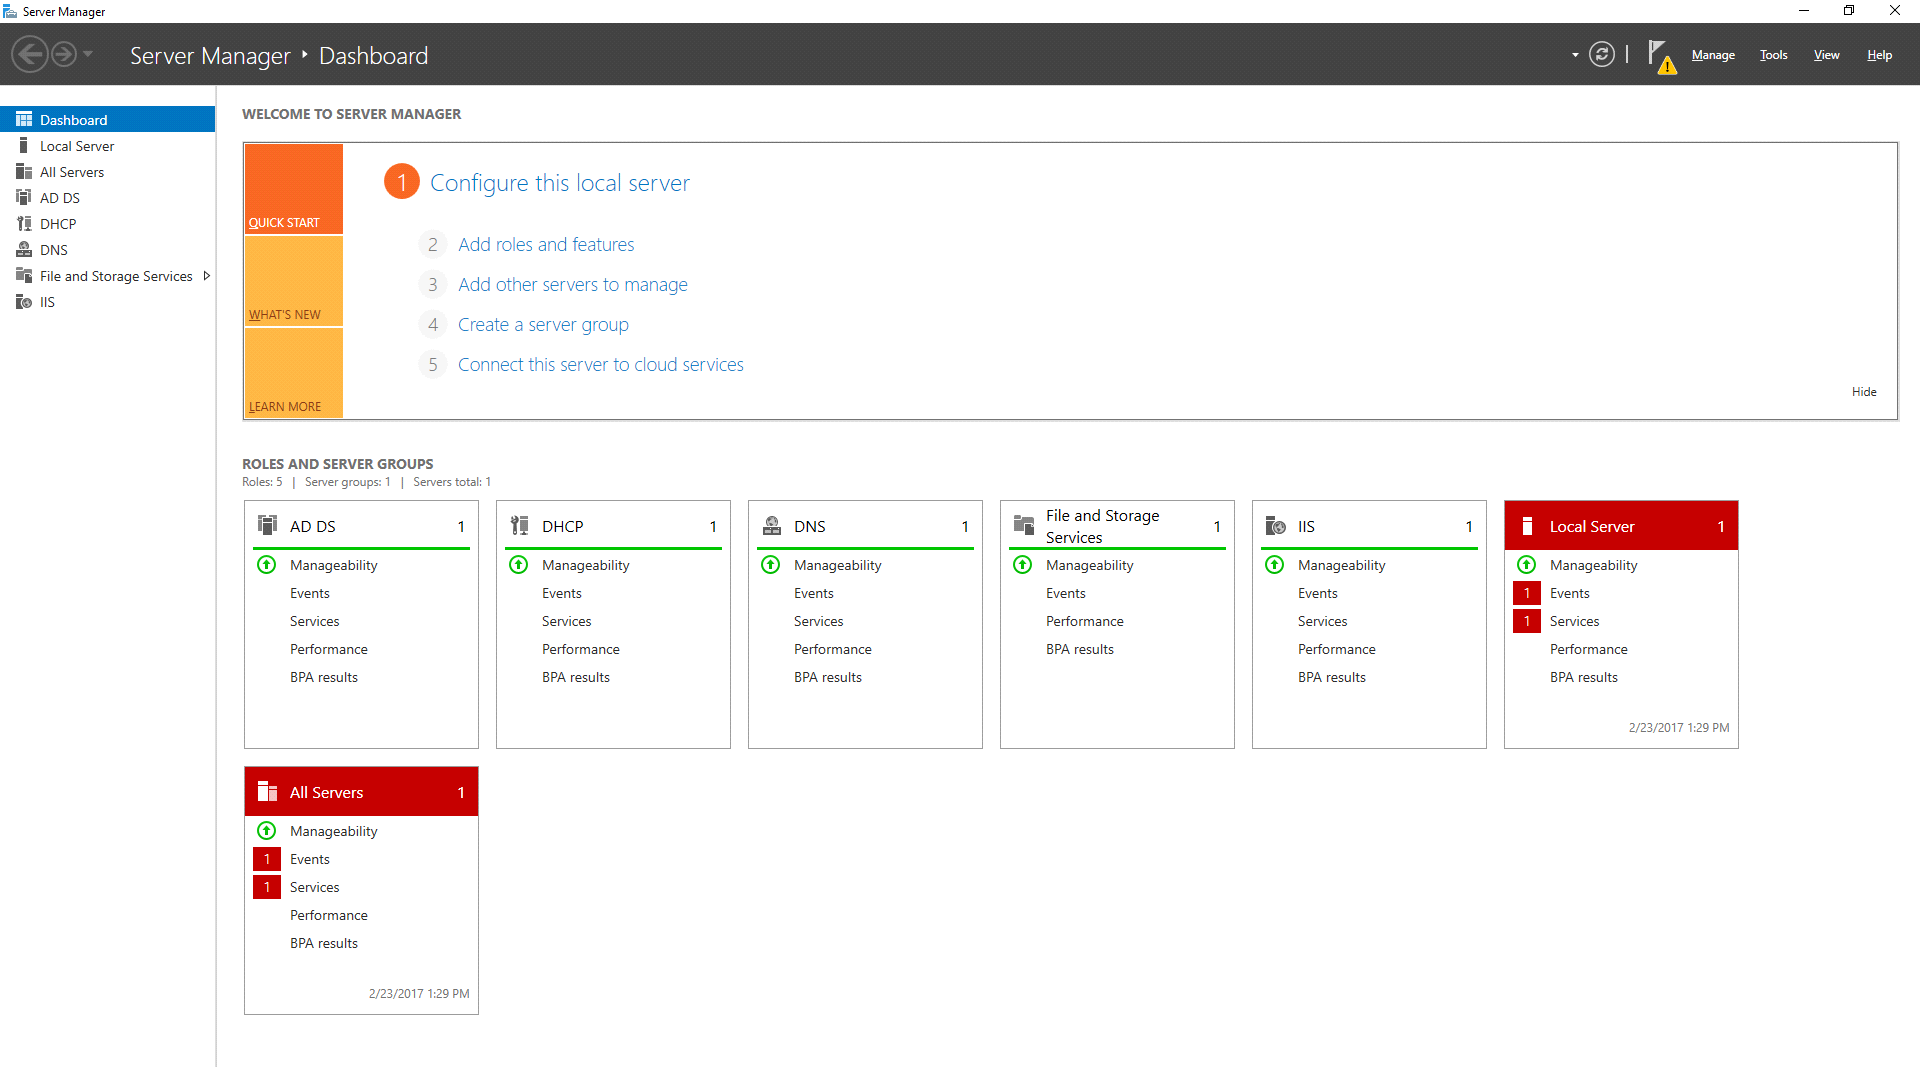
\includegraphics[scale=0.3]{win_priprava}
\caption{Server Manager}
\label{fig:x win_server_man}
\end{figure}

\begin{figure}[!htb]
\centering
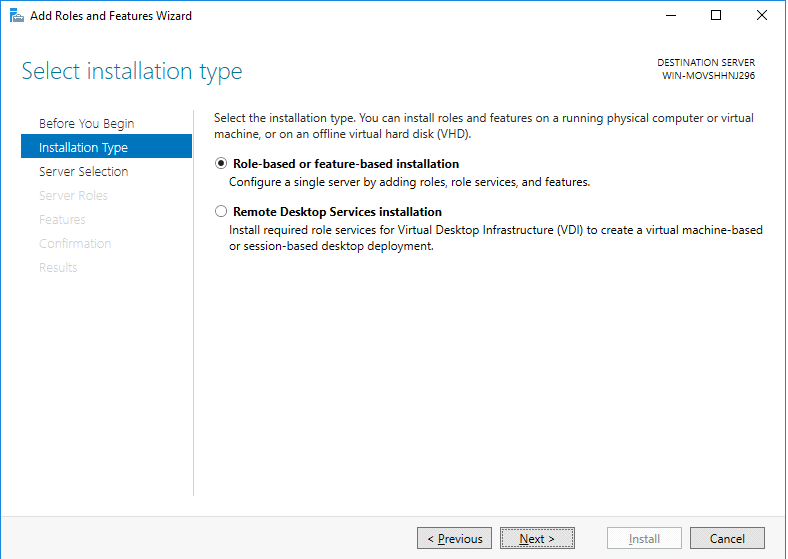
\includegraphics[scale=0.7]{win_priprava_2}
\caption{Inštalácia DHCP, DNS a IIS}
\label{fig:x win_prep_2}
\end{figure}

\begin{figure}[!htb]
\centering
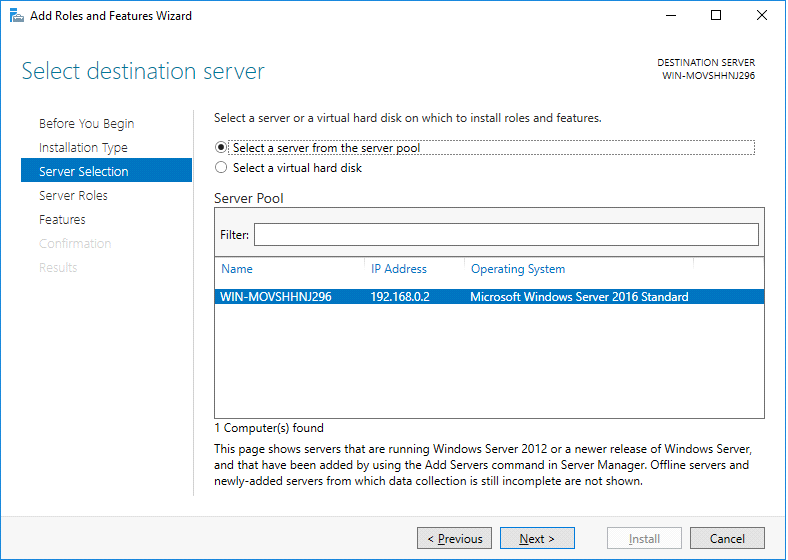
\includegraphics[scale=0.7]{win_priprava_3}
\caption{Spôsob inštalácie novej role pre Windows Server}
\label{fig:x win_prep_3}
\end{figure}

\begin{figure}[!htb]
\centering
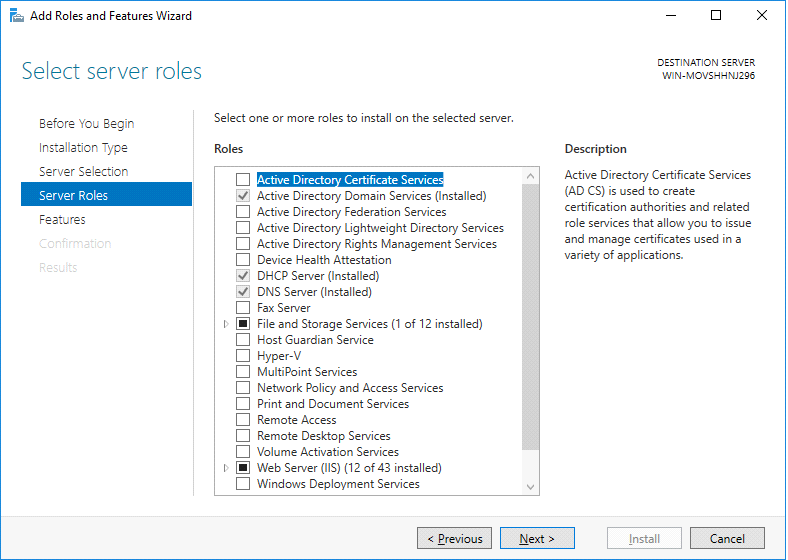
\includegraphics[scale=0.7]{win_priprava_4}
\caption{Nainštalované role pre systém Windows Server}
\label{fig:x win_prep_4}
\end{figure}

\section{Základná konfigurácia}
\paragraph{}
Do Windows Server-u 2016 sme nainštalovali webový prehliadač Mozilla Firefox alebo Google Chrome (podľa preferencie - Internet Explorer bol prakticky nepoužiteľný). Podobne ako Windows 10, aj Windows Server 2016 inštaluje aktualizácie automaticky, pričom sa aktualizácie inštalujú do systému samé od seba, bez vedomia administrátora. Preto sme sa rozhodli automatické aktualizácie vypnúť priamo v nastavení služieb systému Windows. Konkrétne sme vypli službu \say{Windows Update} tým, že sme jej stav nastavili na \say{Disabled}. Po nastavení sme reštartovali servery.

\section{DNS}
\paragraph{}
V prvom rade sme si zvolili Master a Slave. Master je server1 (192.168.0.2) a Slave server2 (192.168.0.3)
\paragraph{}
DNS master nainštalujeme pomocou Windows Server Manager. Klikneme na Manage , vyberieme možnosť Add roles and features daľej Role-based or feature-basedinstallation, zobrazí sa  zoznam serverov, my vyberieme náš server a zvolímezo zoznamu rolesDNS Server a dokončíme inštaláciu.
\paragraph{}
Po inštalácií DNS balíka sme sa dostali cez Tools -\textgreater{} DNS -\textgreater{} Configure a DNS server -\textgreater{} Create a forward lookupzone k vytvoreniu primárnej forward lookupzóny sos1.local , nastavili sme aj  nech záznamy preposiela na Slave 192.168.0.3.
\paragraph{}
Prešli sme k inštalácii DNS Slave.Postup ako pri DNS Master avšak  DNS server bolo potrebné nastaviť na slavemode. Vybrali sme  Tools -\textgreater{} Forward lookupzones -\textgreater{} New zone. Hneď v prvom kroku sme vybrali  možnosť nie Primaryzone ale Secondaryzone a taktiež  meno zóny .V ďalšom kroku určíme DNS Masterserver,v našom riešení ma  IP 192.168.0.2 .Dokončíme vytváranie zóny pomocou Next a Finish. Onedlho si Slave stiahne záznamy z DNS Master servera.

\begin{figure}[!htb]
\centering
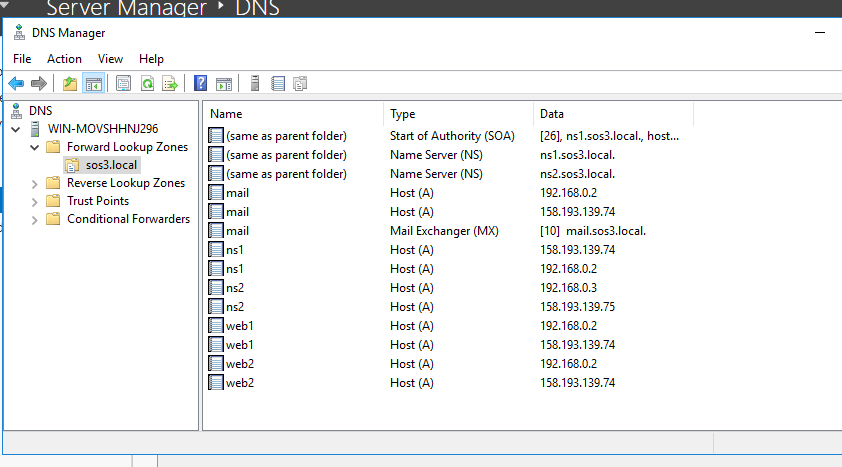
\includegraphics[scale=0.7]{win_dns_win_zaznamy}
\caption{DNS záznamy}
\label{fig:x win_dns}
\end{figure}

\section{DHCP}
\paragraph{}
Inštaláciu sme vykonali vo Windows service manager - Add Roles and Features, vybrali si možnosť DHCP server.
\paragraph{}
Pre konfiguráciu sme klikli na TOOLS a následne DHCP.Zobrazilo sa nám okno s ponukou , my sme vybrali náš server, IPv4 a možnosť new scope. Spustil sa New ScopeWizard. V prvom kroku  sme napisali názov pravidla na prideľovanie IP adries. Ďalej sme zvolili  rozsah IP adries a masku.
\\
\\
Rozsah IP adries od 192.168.0.1 po 192.168.0.254\\
Maska 255.255.255.0
\paragraph{}
Následne sme využili možnosti pridať výnimku z predtým zadaného rozsahu, teda adresy ktoré sa nebudu prideľovať napriek tomu, že sú zo nami  zadaného rozsahu v predchádzajúcom kroku. Ide o adresy serverov 192.168.0.2 a 192.168.0.3.
\paragraph{}
Potom  sme zvolili aký dlhý čas si server bude pamätať IP adresy ktoré niekomu pridelil. Stačilo nám 5 hodín (dĺžka cvičenia aj s rezervou).
\paragraph{}
Nakoniec sme nastavili bránu na „192.168.1.1”, pridali sme IP adresy našich DNS serverov, teda  „192.168.1.2“ a „192.168.1.3”. , a dokončili inštaláciu kliknutím na Finish.

\begin{figure}[!htb]
\centering
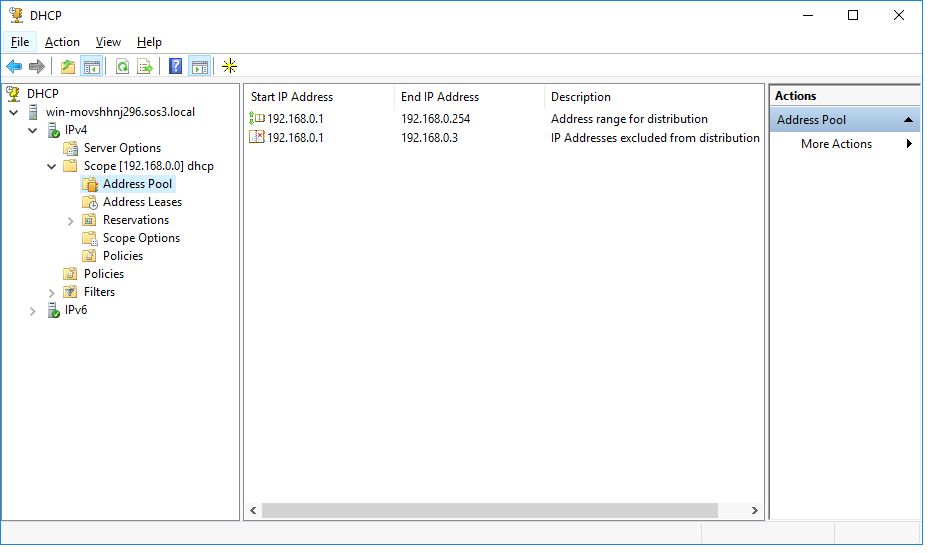
\includegraphics[scale=0.6]{win_dhcp_win_pool}
\caption{Konfigurácia DHCP}
\label{fig:x win_dhcp_pool}
\end{figure}


\section{NTP}
\paragraph{}
Na spustenie NTP na Windows servery sme museli vykonať zmeny v registroch. Spustíme okno RUN  (WIN+R) , kde napíšeme regedit. Následne sa dostaneme cestou HKEY\_LOCAL\_MACHINE | SYSTEM | CurrentControlSet | Services | W32Time | TimeProviders | NtpServer	až k hodnote Enabled , ktorá bola nastavená na 0 , a my ju zmeníme na 1.Využijeme opäť win+R , zadáme w32tm /config /update,čím vlastne spustíme NTP server na danom zariadení.
\paragraph{}
Na aplikáciu  zmien sme reštartovali Windows Timeservice príkazom zadaným do commandline:
\\
\\
net stop w32time \&\& net start w32tim.

\section{Web server}
\paragraph{}
Webserver IIS (Internet Information Server) sme pridali cez windows server manager tlačidlom Addroles and features, kde sme vyhľadali Web Server ISS a pokračujeme ďalej. Pri ponuke Role Services
\paragraph{}
Následne nainštalujeme služby na server. Po úspešnej inštalácii sa IIS objaví na \v{l}avom paneli v server manager-i. Klikneme na ikonu IIS a v zozname dostupných serverov sa zjaví jeden - ten, na ktorom uskuto\v{c}\v{n}ujeme konfiguráciu. Klikneme na\v{n} pravým tla\v{c}idlom myši a z ponuky zvolíme možnos\v{t} Internet Information Services (IIS) Manager. Otvorí sa nové okno, v ktorého \v{l}avom paneli sa nachádza náš server. Rozbalíme jeho ponuku a klikneme na Sites. Pravý klik na Default Web Site nám ponúkne viacero možností vrátane nastavenia webstránky a pridania novej.

\paragraph{}
Po inštalácii sa nachádza ISS v ľavom paneli vo Windows Server Manager-i. Po kliknutí na tools v pravom hornom rohu klikneme Internet Information Services (ISS) manager. A po rozkliknutí na ľavom rohu je už vytvorená default sites. Otvoriť ju je možné zadaním do browseru “localhost”.

\begin{figure}[!htb]
\centering
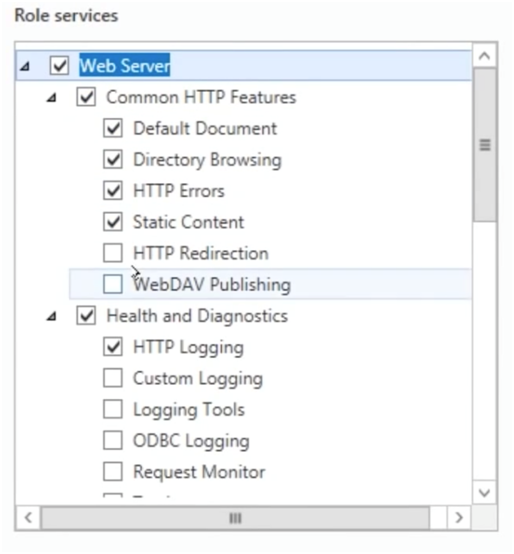
\includegraphics[scale=0.79]{win_iis_web_server}
\caption{Inštalácia webového servera IIS}
\label{fig:x win_web}
\end{figure}

\begin{figure}[!htb]
\centering
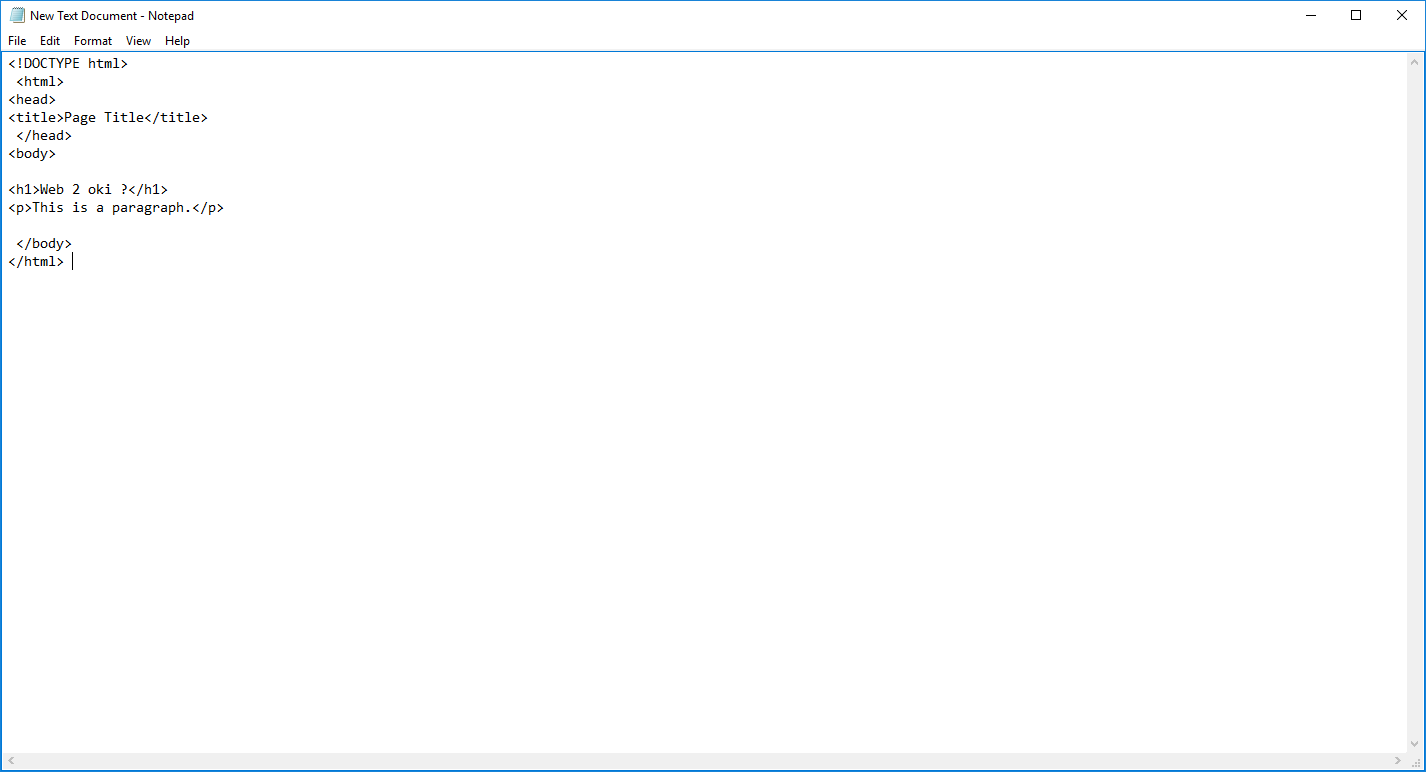
\includegraphics[scale=0.5]{win_iis_web2}
\caption{Zdrojový kód stránky "web2"}
\label{fig:x win_web2_source}
\end{figure}

\begin{figure}[!htb]
\centering
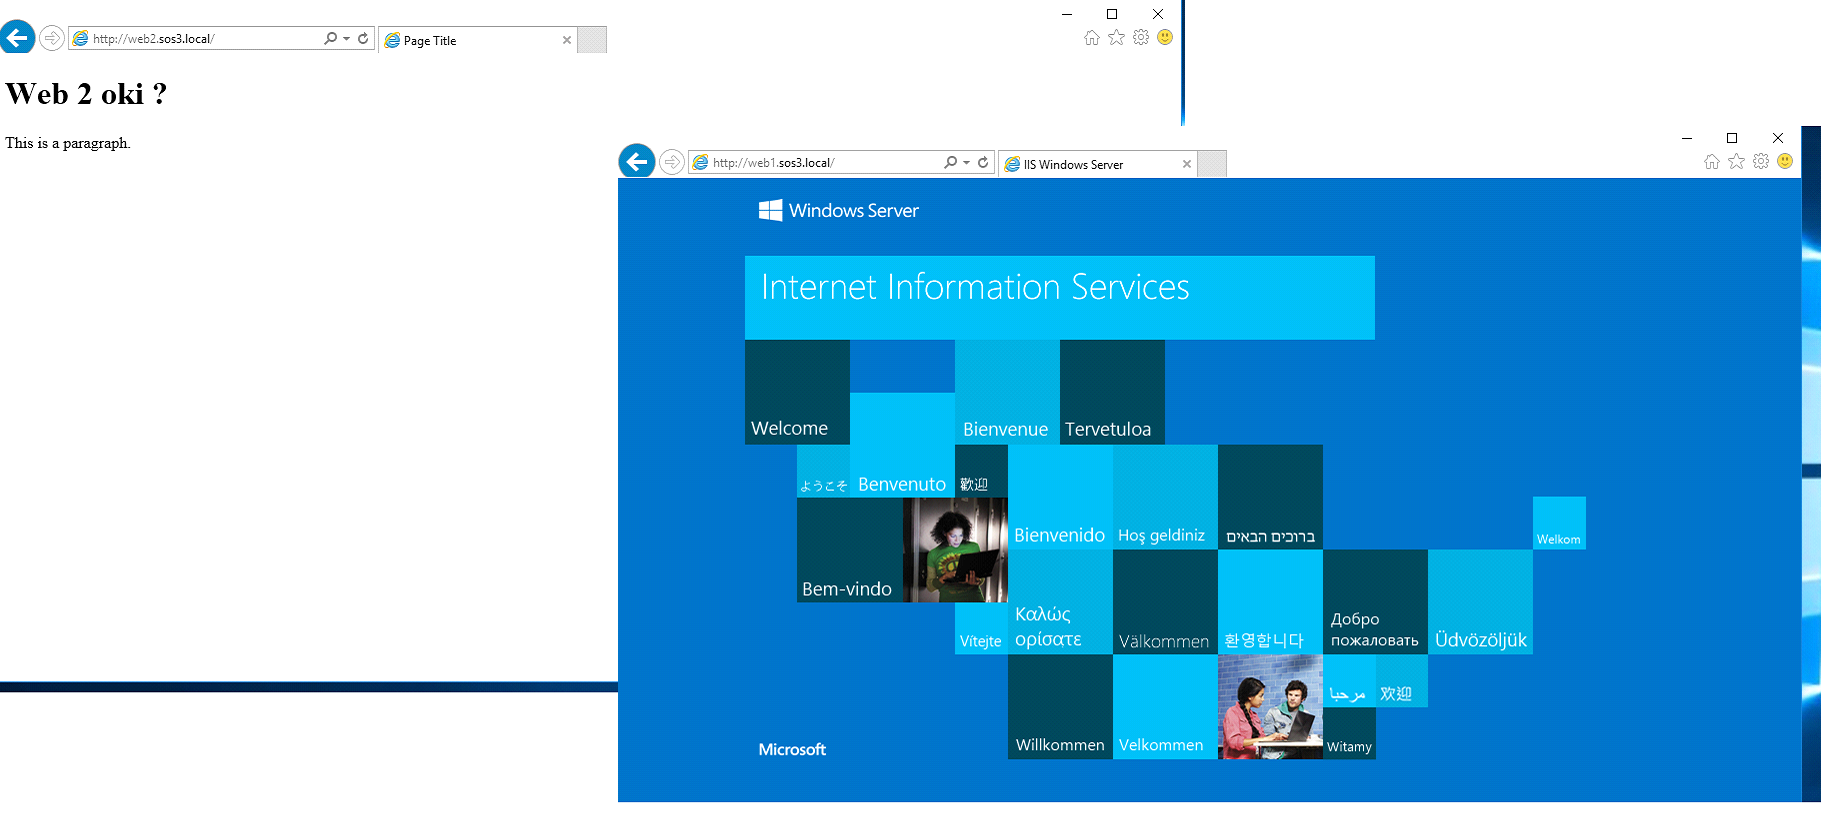
\includegraphics[scale=0.4]{win_iis_web1_web2}
\caption{Ukážka webových stránok "web1" (vpravo) a "web2" (vľavo)}
\label{fig:x win_web}
\end{figure}

\section{Poštový server}
\paragraph{}
V server manageri klikneme na tools a v záložne DNS, nasmerujume sa ku DNS severu a vytvoríme nové záznamy pre mail server. Cname záznam mail 158.193.139.74, dva MX(Mail exchanger) záznamy 0 mail sos3.local a 10 mail sos3.local.
\paragraph{}
Zo stránky mailenable.com stiahneme standart edition. Začneme inštaláciou stiahnutého balíčka, zaklikneme web mail service(server). V nasledujúcich krokoch napí\-šeme do Domain Name: sos3.local a DNS host: 192.168.0.2 a smtp port: 25. Počas inštalácie nám vybehne tabuľká, kde odklikneme aby sa mailserver inštaloval ako webserver ISS. V server manageri po kliknutí servers -\textgreater{} localhost -\textgreater{} system -\textgreater{} diagnose si skontrolujeme či všetky políčka sú pass, čo nám značí že mail enable funguje. V ďalšom kroku servers -\textgreater{} localhost -\textgreater{} services and connectors  a na SMTP klikneme pravým tlačidlom a klikneme na properties. V záložne general nastavíme default mail domain name čo je v našom prípade mail.sos3.local. Ďalej v záložke smart host nastavíme IP/DOMAIN 158.193.139.74. Po reštarte serveru vidíme že, všetky service sú running.

\begin{figure}[!htb]
\centering
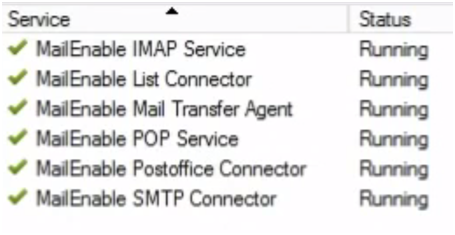
\includegraphics[scale=0.79]{win_mail_server}
\caption{Inštalácia poštového servera MainEnable}
\label{fig:x win_mail}
\end{figure}

\section{NAT}
\paragraph{}
Inštaláciu sme vykonali vo Windows Server Manageri, kde sme cez \say{Add Roles and Features} pridali službu \say{Routing and Remote Access} a následne sme ju nainštalovali. Pri inštalácii zvolíme sie\v{t}ový adaptér eth0, ktorý je pripojený k internetu. Po inštalácii je NAT plne funkčné, ale je potrebné prida\v{t} NAT záznamy na porte 53 pre tcp aj udp.  Ďalej sme potrebovali nakonfigurovať NAT v Control Panel -\textgreater{} Administrative tools -\textgreater{} Routing and Remote Access. Po kliknutí na NAT, vyberieme záložku s adaptérom, ktorý je pripojený k internet. V Address Pool je potrebné nastavi\v{t} položku \say{from}, čo znamená náš rozsah verejných adries 158.193.139.74 a to, čo je naša koncová adresa 158.193.139.75 a maska 255.255.255.252. V záložke services and ports je potrebné prida\v{t} 4 nové záznamy NAT pre DNS(Master-Slave, TCP-UDP).

\begin{figure}[!htb]
\centering

\includegraphics[scale=0.79]{win_iis_remote_access}
\caption{Povolenie vzdialeného prístupu}
\label{fig:x win_web}
\end{figure}
